\documentclass{beamer}

\usepackage[english]{babel}
\usepackage[letterpaper,top=2cm,bottom=2cm,left=3cm,right=3cm,marginparwidth=1.75cm]{geometry}
\usepackage{amsmath}
\usepackage{graphicx}
\usepackage{float}
\usepackage{subcaption}
\usepackage[colorlinks=true, allcolors=blue]{hyperref}


\usepackage[
  backend=biber,
  style=alphabetic,
  sorting=ynt
]{biblatex}
\addbibresource{SPCSimLib.bib}

\title{Determining the accuracy of SPC Pictures taken using Equi-Width Histograms versus Equi-Depth Histograms, Parallel versus Asynchronous Data Collection and 1.5 FWHM versus 5.0 FWHM under variable Attenuation using SPCSimLib \cite{spc}}
\author{Elliott H. VanOrman, Intern at the Institute for Computing in Research, working for Professor Atul Ingle and Kaustubh Sadekar}

\begin{document}

\maketitle

\begin{frame}
  \center{\bfseries{INTRODUCTION}}
\end{frame}

\begin{frame}
  These slides tell the story of how I compared the error in results of a Single Photon Camera (SPC) when using Equi-Width Histograms (EWH) versus Equi-Depth Histograms (EDH), parallel versus asynchronous data collection, and 1.5 FWHM versus 5.0 FWHM laser pulses.
  Data was collected using the python library SPCSimLib, specifically by simulating a single SPC pixel, and measuring the error each method produced.
  My analysis showed using Equi-Width Histograms, asynchronous data collection, or 1.5 FWHM pulses creates pictures matching reality more closely than those created using Equi-Depth Histograms, parallel data collection, or 5.0 FWHM pulses, to a statistically significant level.
  From this, I concluded that using Equi-Width Histograms, Asynchronous data collection and 1.5 FWHM pulses produces more accurate results than using Equi-Depth Histograms, Parallel data collection, and 5.0 FWHM pulses.
\end{frame}

\begin{frame}
  \center{\bfseries{BACKGROUND INFORMATION}}
\end{frame}

\begin{frame}
  Single Photon Cameras, or 'SPC's for short, are cameras that function similarly to LIDAR, in that they produce 3D photographs by measuring the time it takes for light to travel to a point and bounce back. Unlike LIDAR however, SPCs use individual photons instead of lasers. \cite{ingle} \cite{sadekar}
  
  When a picture is taken, the SPC begins sending out pulses of photons towards the thing it is taking a picture of. When these photons are reflected back onto the detector, it records the timestamp. We can then calculate the distance away from our camera using the formula\[\frac{T*\frac{1}{2}}{C}\] where $T$ is the time it took photons to reflect back to the detector and $C$ is the speed of light. \cite{sadekar}
\end{frame}

\begin{frame}
  \begin{figure}[H]
    \centering
    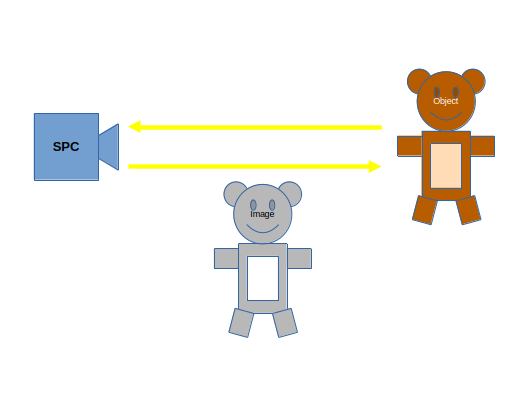
\includegraphics[width=1\linewidth]{SPCExplained.png}
    \caption{\label{fig:Data}How SPCs Work.}
  \end{figure}
\end{frame}

\begin{frame}  
  There are almost always ambient photon levels, however, meaning that while timestamps do cluster around the 'true' time it took photons to reflect back, there are always a few 'noise' timestamps due to background illumination. They can be minimized via turning off lights and waiting for nightfall, but this is often not enough. There are multiple methods to determine when the true center of the pulse (called the 'peak') is located. After the 'peak' is located, it is used as $T$ in the previously shown formula \cite{sadekar}.
\end{frame}

\begin{frame}
  Taking an accurate picture, collecting data accurately, and sorting the noise from the real data is quite complicated however, and there are several factors to consider. Namely:
  \begin{itemize}
  \item The kind of histogram used to locate the peak.
  \item Whether collectors collect data asynchronously or in parallel.
  \item How long the laser fires.
  \end{itemize}
\end{frame}

\begin{frame}  
  There are two types of histograms to use when finding the peak: \cite{sadekar}
  \begin{itemize}
  \item Equi-Width Histograms, histograms with buckets of equal width but variable depth. For EWHs, The 'peak' bucket is the bucket with most detections.
  \item Equi-Depth Histograms, histograms with buckets of variable width but equal depth. For EDHs, the 'peak' bucket is the bucket of the shortest width.
  \item In both cases, The center of the 'peak' bucket is recorded as the 'peak' of the pulse.
  \end{itemize}
\end{frame}

\begin{frame}
  \begin{figure}[H]
    \centering
    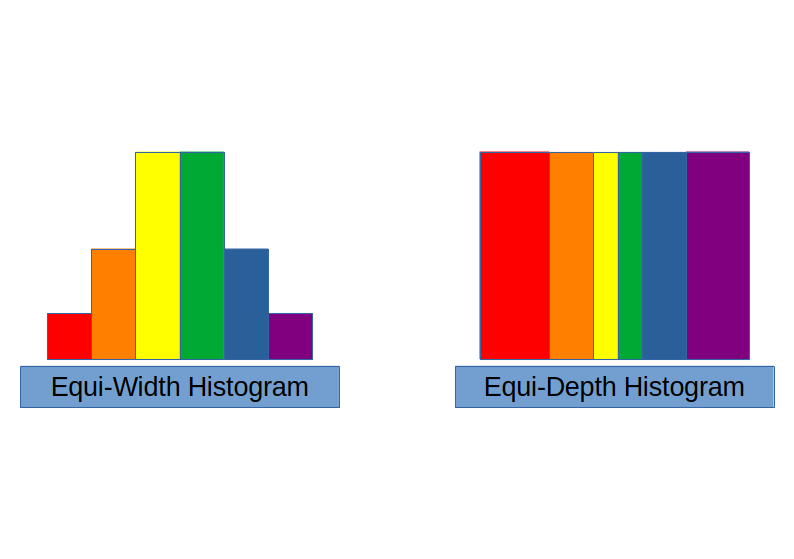
\includegraphics[width=1\linewidth]{Histograms.png}
    \caption{\label{fig:Data}The two kinds of histogram.}
  \end{figure}
\end{frame}

\begin{frame}
  Before I explain the difference between asynchronous mode and parallel mode, I first need to explain deadtime.
  \begin{itemize}
  \item Due to the physical limitations of SPC cameras photon readings over time do not always match reality.
  \item When a detector is hit by a photon, it takes a certain amount of time for said detector to log a timestamp.
  \item While this time is in progress, the detector cannot record new hits. In other words, a detector cannot start recording a new timestamp until it has finished recording the first.
  \item photons that hit the detector during that recording time go undetected.
  \item This time is usually around 75ns in real life, and is refered to as 'deadtime' \cite{sadekar}
  \end{itemize}
\end{frame}

\begin{frame}
  There are two modes in which one collects data: \cite{sadekar}
  \begin{itemize}
  \item Parallel (or, Not Freerun) Mode. In Parallel mode, detectors are reset at the beginning of each pulse, resetting their deadtime, but skewing timestamps to the right as early photons will block later photons
  \item Asynchronous (or, Freerun) Mode. In Asynchronous mode, detectors are simply allowed to run, their deadtime elapsing in full but leaving their timestamps less skewed.
  \end{itemize}
\end{frame}

\begin{frame}
  Then there is FWHM:
  \begin{itemize}
  \item FWHM, unlike histograms and modes, is a continous measurement of how long each laser pulse fires.
  \item FWHM, or Full Width at Half Maximum, refers to the length of the curve of intensity of the laser when it fires. It can also affect the error of the laser, as the increaed length of the laser would also increase the width of the 'peak' of the pulse.
  \end{itemize}
\end{frame}

\begin{frame}
  \begin{itemize}
  \item Unfortunately, due to the skew in data, it often becomes necesary to filter out a certain percent of incoming photons.
  \item This filtering is called 'attenuation' \cite{ingle}, and it does reduce the overal number of photons hitting an SPC.
  \item Because of the fact that any one datapoint blocks other datapoints from being recorded for a period of time causes it to actually increase the amount of photons not blocked by early recordings.
  \item this reduces the skew of the timestamp data and increasing accuracy. \cite{sadekar}
  \end{itemize}
\end{frame}

\begin{frame}
  this matters because there are many methods that can be used to receive and interpret data from SPCs, but it has not yet been determined which produces the most accurate results.
  I hypothesized that...
  \begin{itemize}
  \item Equi-depth histograms would produce more accurate results than Equi-Width histograms.
  \item asynchronous (non-freerunning) mode would produce more accurate results than parallel (freerunning) mode.
  \item 1.5 FWHM would produce the same amount of error as 5.0 FWHMs.
  \end{itemize}
\end{frame}

\begin{frame}
  \center{\bfseries{METHODS USED TO COLLECT DATA}}
\end{frame}

\begin{frame}
  In order to determine what produced the most accurate results, I used the Python library SPCSimLib \cite{spc} to simulate a pixel of an SPC. To find error, I...
  \begin{enumerate}
  \item Simulated taking a picture with the pixel.
  \item Subtracted the 'true distance' (the real distance from the camera in the simulation) from the 'estimated distance' (the distance the camera estimated).
  \item Normalized said distance from -1 to 1 by dividing it by the scale of the distance (tbins). (This normalized difference is what I refer to when I say 'error'.)
  \item Repeated the previous three steps ten times and took the average for each set of values. (to reduce fluctuations)
  \item Repeated the previous four steps one hundred and one times, each time incrementing the attenuation multiplier by 0.01.
  \item Put the resultant data into a file labeled  with the settings the SPC used while simulations were being taken.
  \item then I changed the settings and repeated all previous steps until I had run out of combinations of settings to test.
  \end{enumerate}
\end{frame}

\begin{frame}
  \begin{figure}[H]
    \centering
    \begin{subfigure}[b]{1\textwidth}
      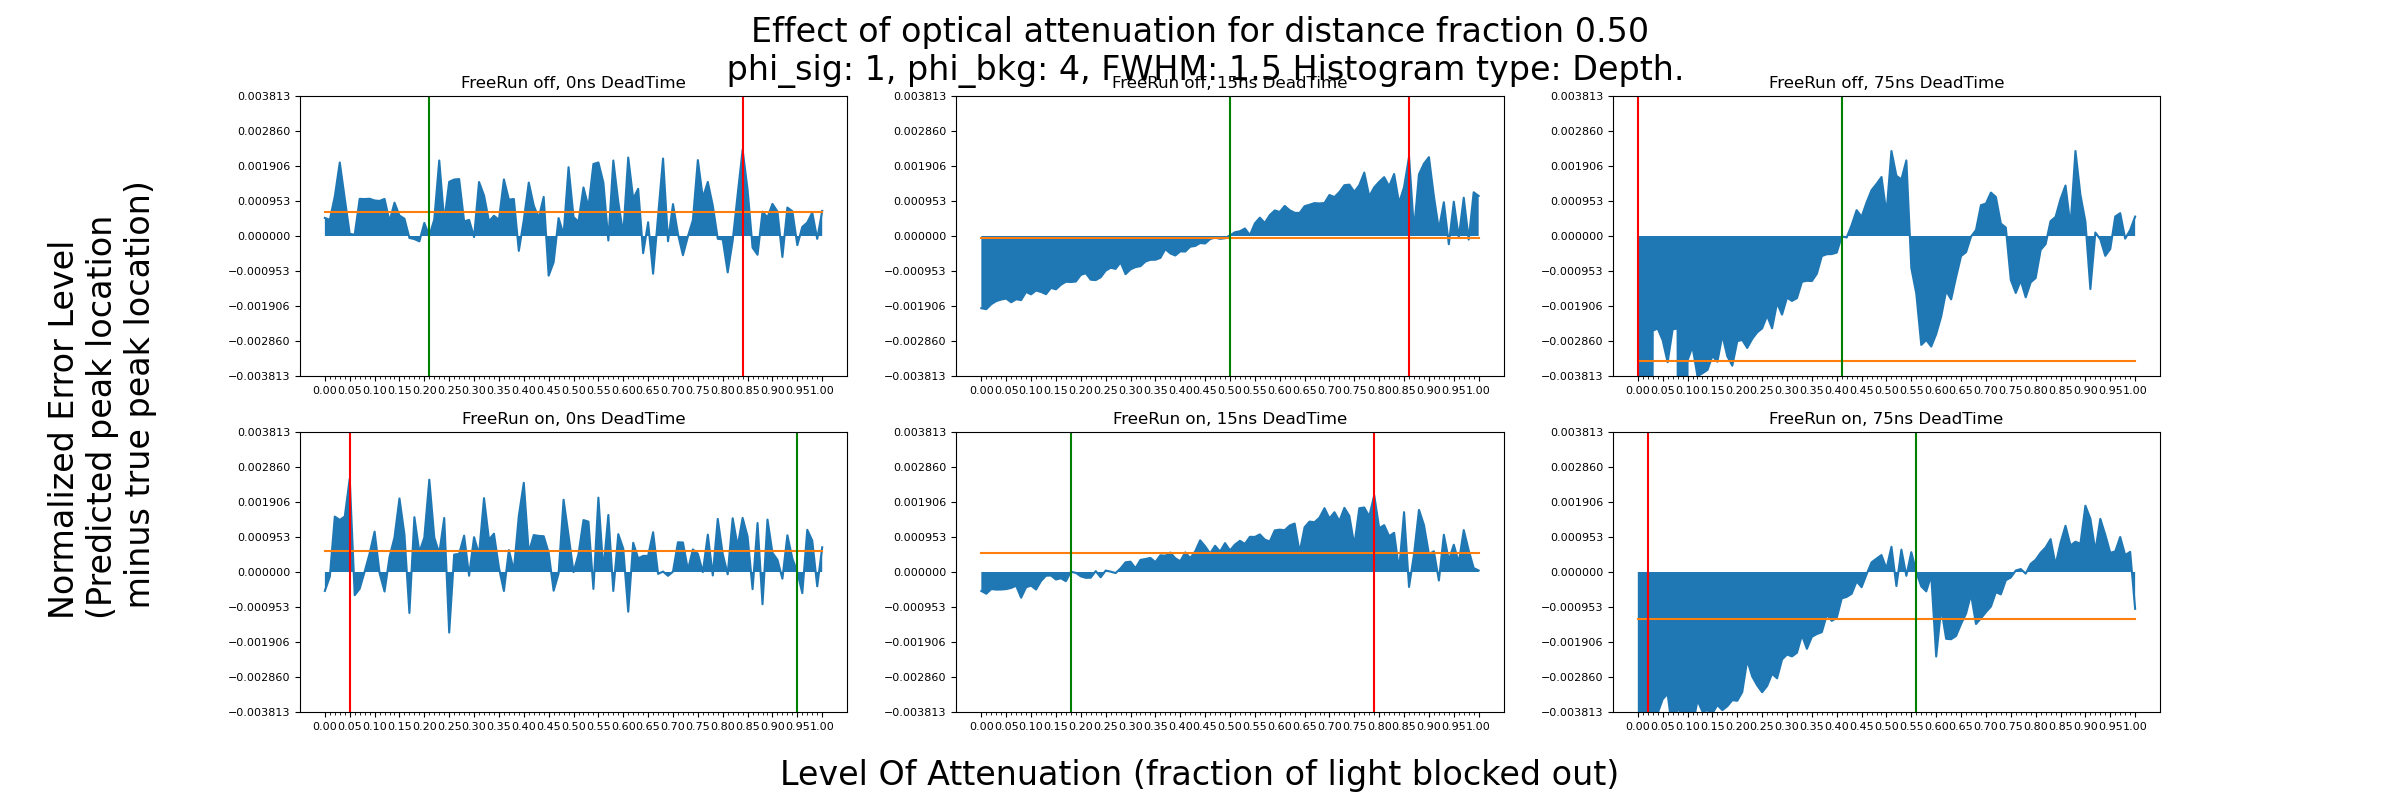
\includegraphics[width=1\linewidth]{SharedyExample.png}
      \label{fig:Ng1}
    \end{subfigure}
    \begin{subfigure}[b]{1\textwidth}
      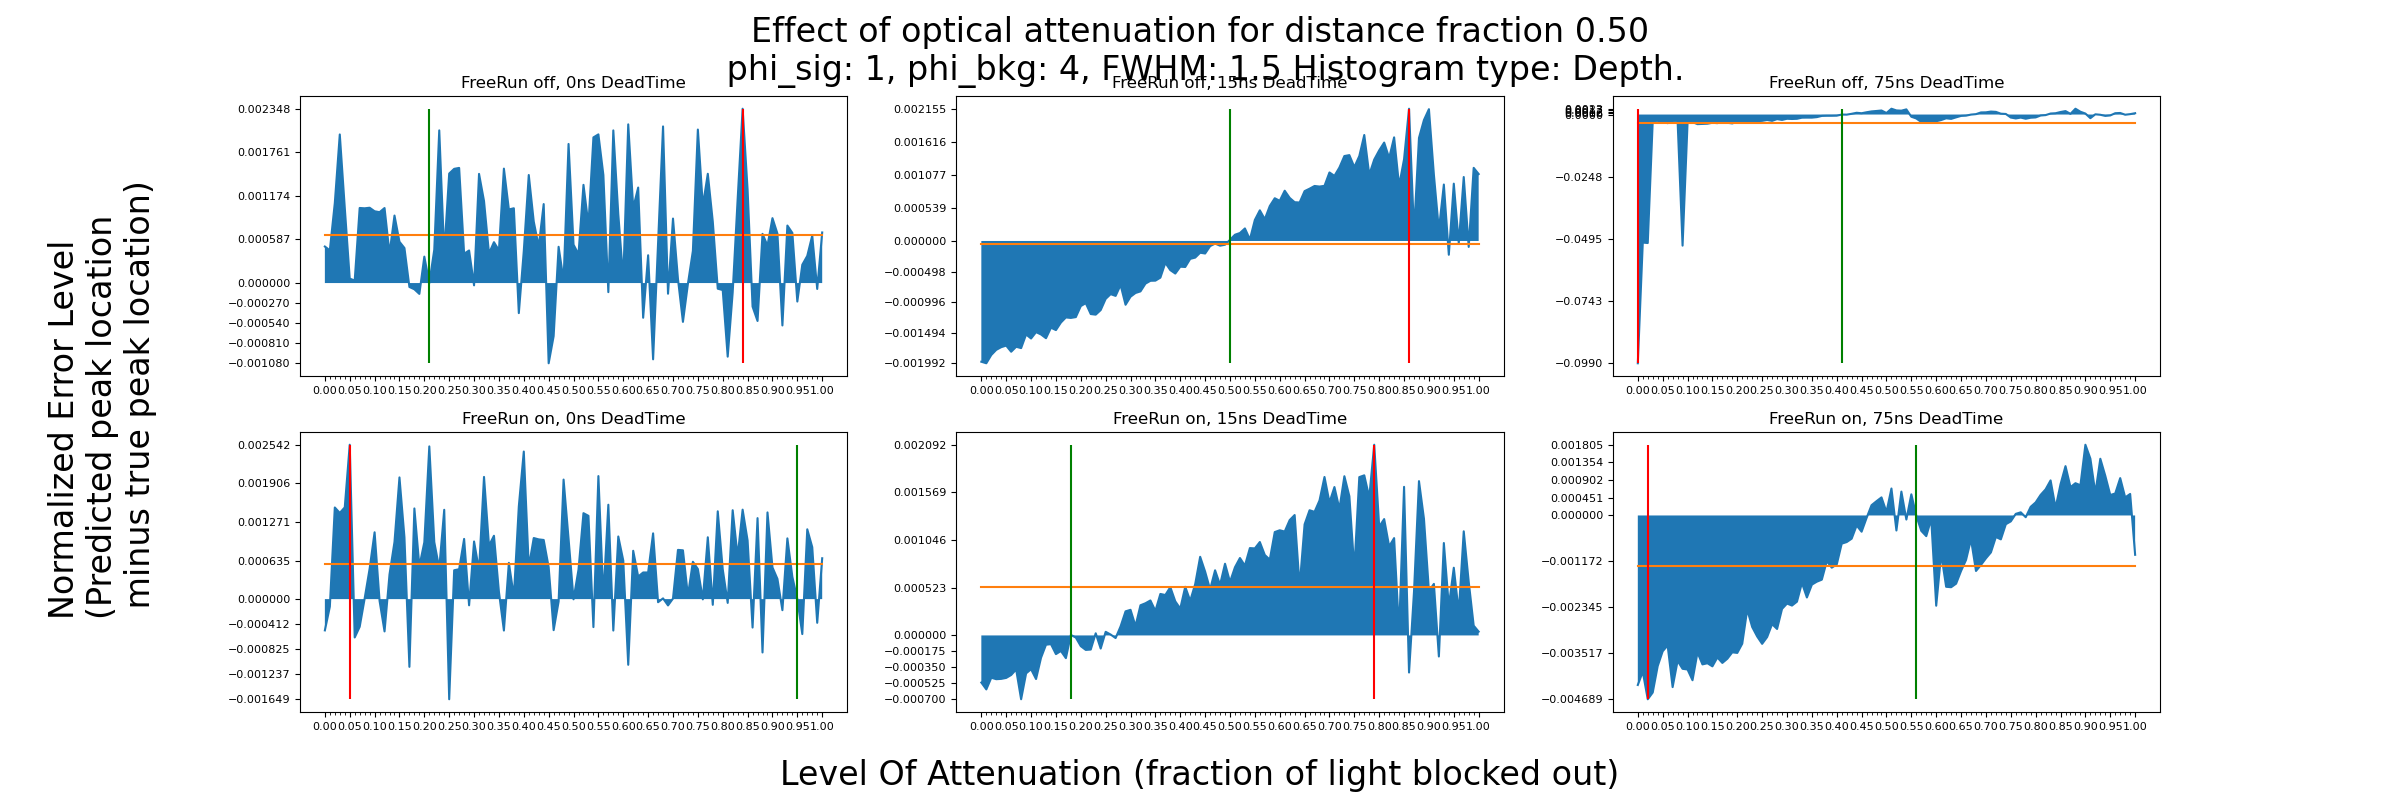
\includegraphics[width=1\linewidth]{ZoomedyExample.png}
      \label{fig:Ng2}
    \end{subfigure}
    \caption{\label{fig:Data}The two formats in which siad data was graphed.}
  \end{figure}
\end{frame}

\begin{frame}
  The top graph and the bottom graph present the same data in two different formats.
  \begin{itemize} 
  \item The top graph represents error on the same scale across all graphs.
  \item The bottom represents each dataset with it's own scale.
  \item Blue represents normalized error.
  \item Orange is the mean error for all attenuation values.
  \item Red is the attenuation value which produced the least accurate result.
  \item Green is the attenuation value which produced the most accurate result.
  \end{itemize}
\end{frame}

\begin{frame}
  in addition, I ran statistical analysis on the data to check my hypotheses. To do this, I put all my data in two large datasets for every hypothesis, one for each differing setting. For every hypothesis, I marked the first dataset $d_{1}$ and the second dataset $d_{2}$. I then performed a paired t-test on the data, where each observation's partner was an observation taken under circumstances identical to the first's except for the variable being tested. 
\end{frame}

\begin{frame}
  \center{\bfseries{RESULTS OF DATA COLLECTION}}
\end{frame}

\begin{frame}
  Using Paired t-tests, I found the following $T$s and P-Values for the following alternate hypotheses:
  \begin{itemize}
  \item $\mu_{EDH}=\mu_{EWH}$: $T=14.59122$
    \begin{itemize}
    \item $\mu_{EDH}>\mu_{EWH}$: $p=1.79689\times10^{-48}$
    \item $\mu_{EDH}\neq\mu_{EWH}$: $p=3.59378\times10^{-48}$
    \item $\mu_{EDH}<\mu_{EWH}$: $p=1.0$
    \end{itemize}  
  \item $\mu_{F}=\mu_{nF}$: $T=-31.63417$
    \begin{itemize}
    \item $\mu_{F}>\mu_{nF}$: $p=1.0$
    \item $\mu_{F}\neq\mu_{nF}$: $p=1.63522\times10^{-218}$
    \item $\mu_{F}<\mu_{nF}$: $p=8.17611\times10^{-219}$
    \end{itemize}
  \item $\mu_{1.5}=\mu_{5.0}$: $T=-55.67372$
    \begin{itemize}
    \item $\mu_{1.5}>\mu_{5.0}$: $p=1.0$
    \item $\mu_{1.5}\neq\mu_{5.0}$: $p=0$
    \item $\mu_{1.5}<\mu_{5.0}$: $p=0$
    \end{itemize}
  \end{itemize}
  I rejected the null for all alternatve hypotheses with p-values less than 0.01. Graphs showing examples of the accepted hypotheses are as follows:
\end{frame}

\begin{frame}
  \begin{figure}[H]
    \centering
    \begin{subfigure}[b]{1\textwidth}
      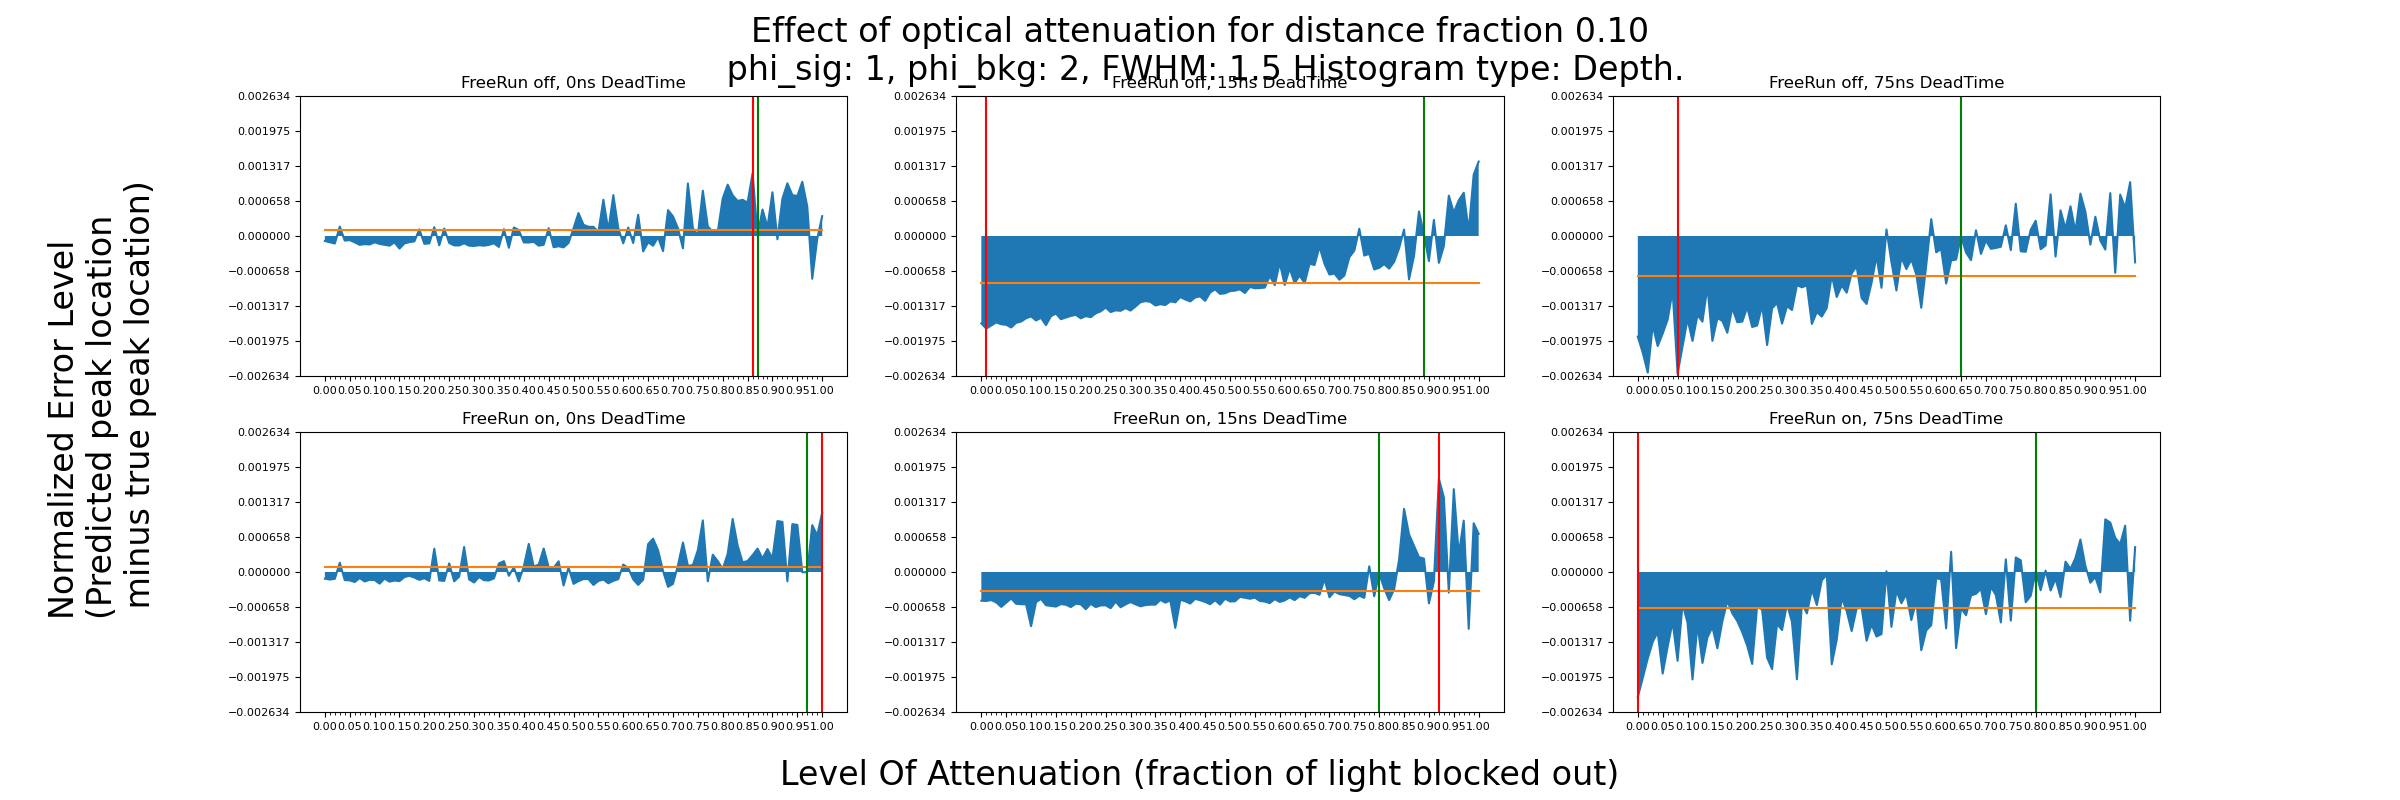
\includegraphics[width=1\linewidth]{depthExample.png}
      \label{fig:Depth Example}
    \end{subfigure}
    \begin{subfigure}[b]{1\textwidth}
      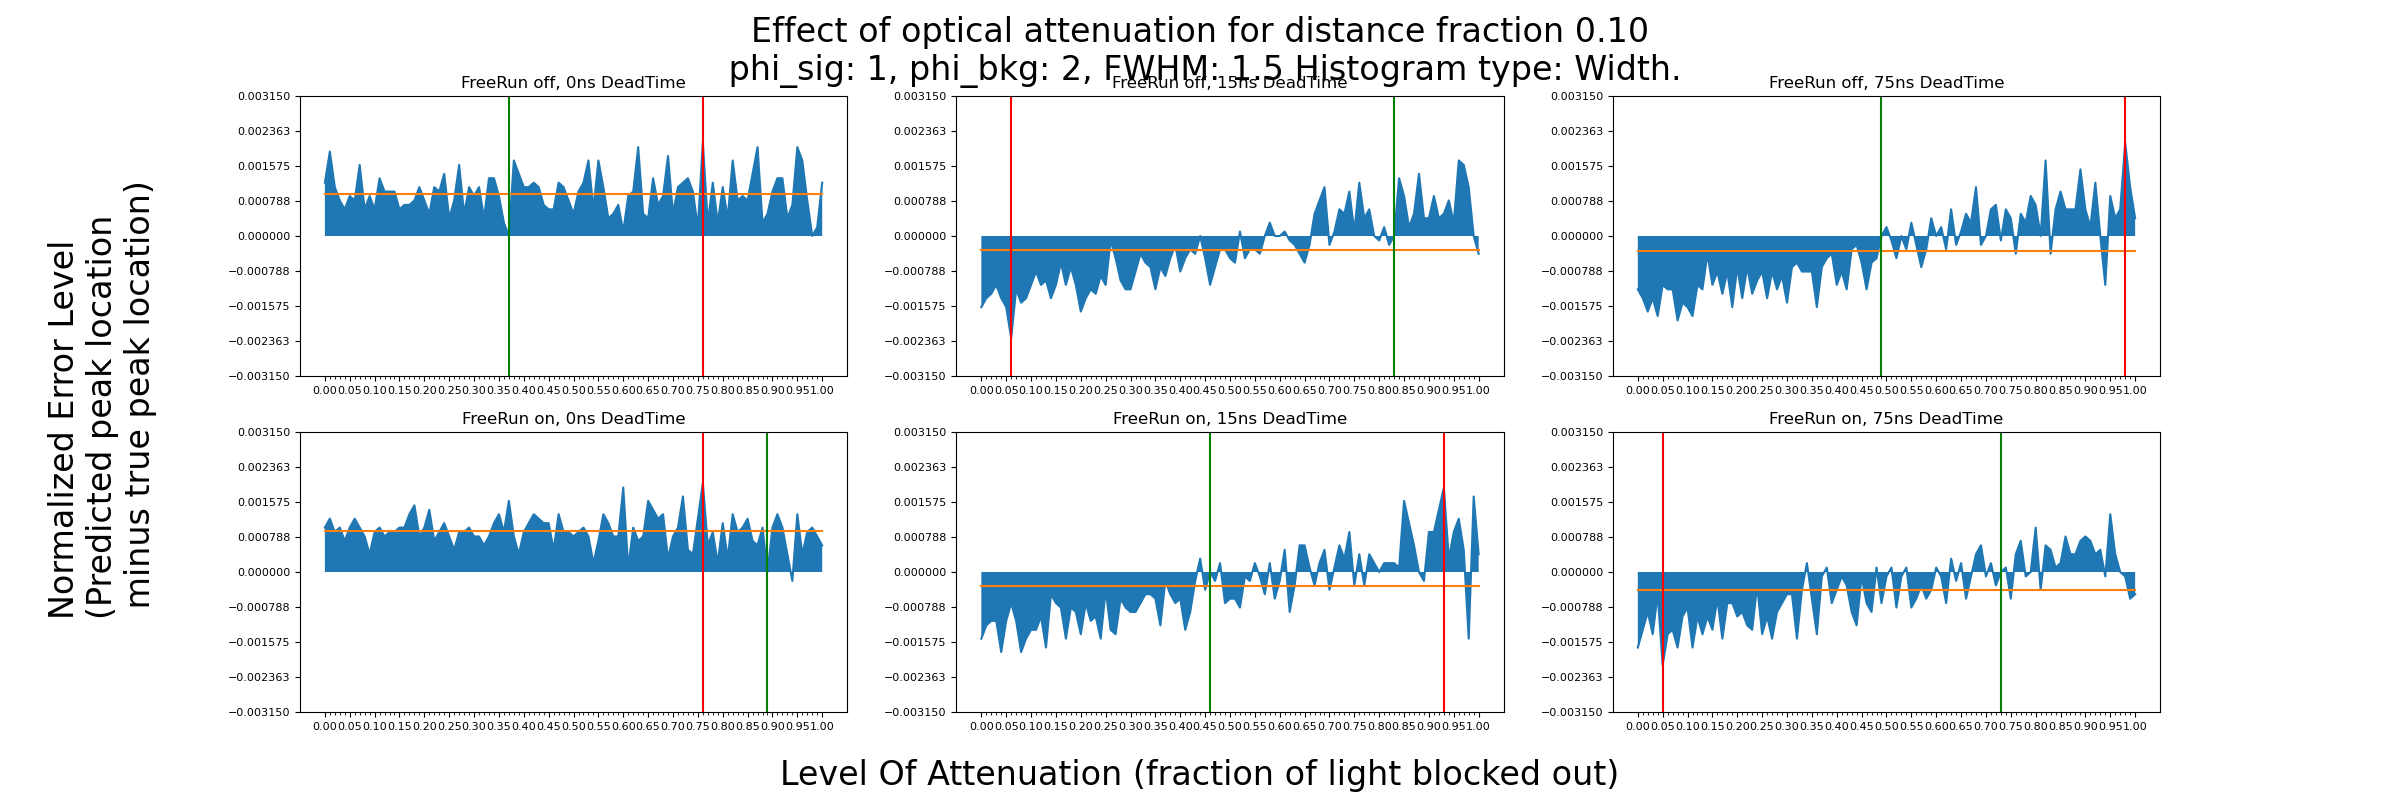
\includegraphics[width=1\linewidth]{widthExample.png}
      \label{fig:Width Example}
    \end{subfigure}
    \caption{\label{fig:histogramComparison}EDH vs EWH}
  \end{figure}
\end{frame}

\begin{frame}
  \begin{figure}[H]
    \centering
    \begin{subfigure}[b]{1\textwidth}
      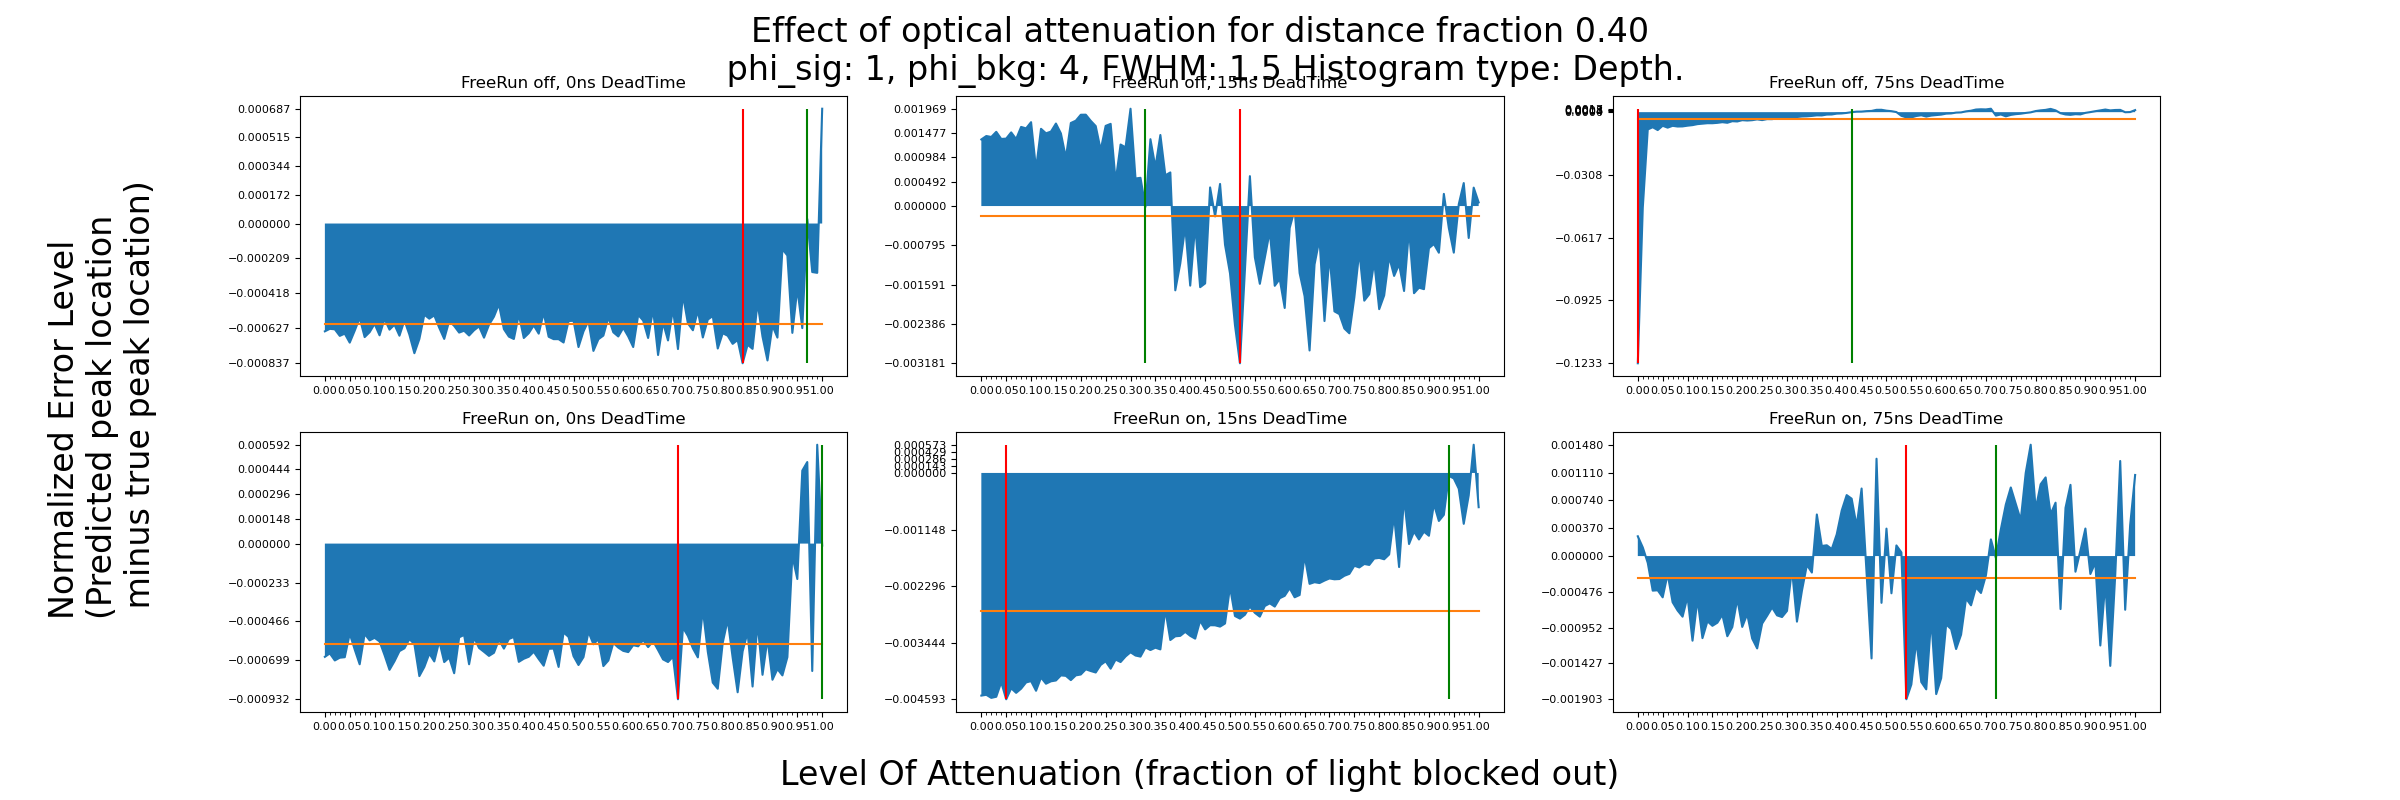
\includegraphics[width=1\linewidth]{zoomedFreeExample.png}
      \label{fig:zoomedExample}
    \end{subfigure}
    \begin{subfigure}[b]{1\textwidth}
      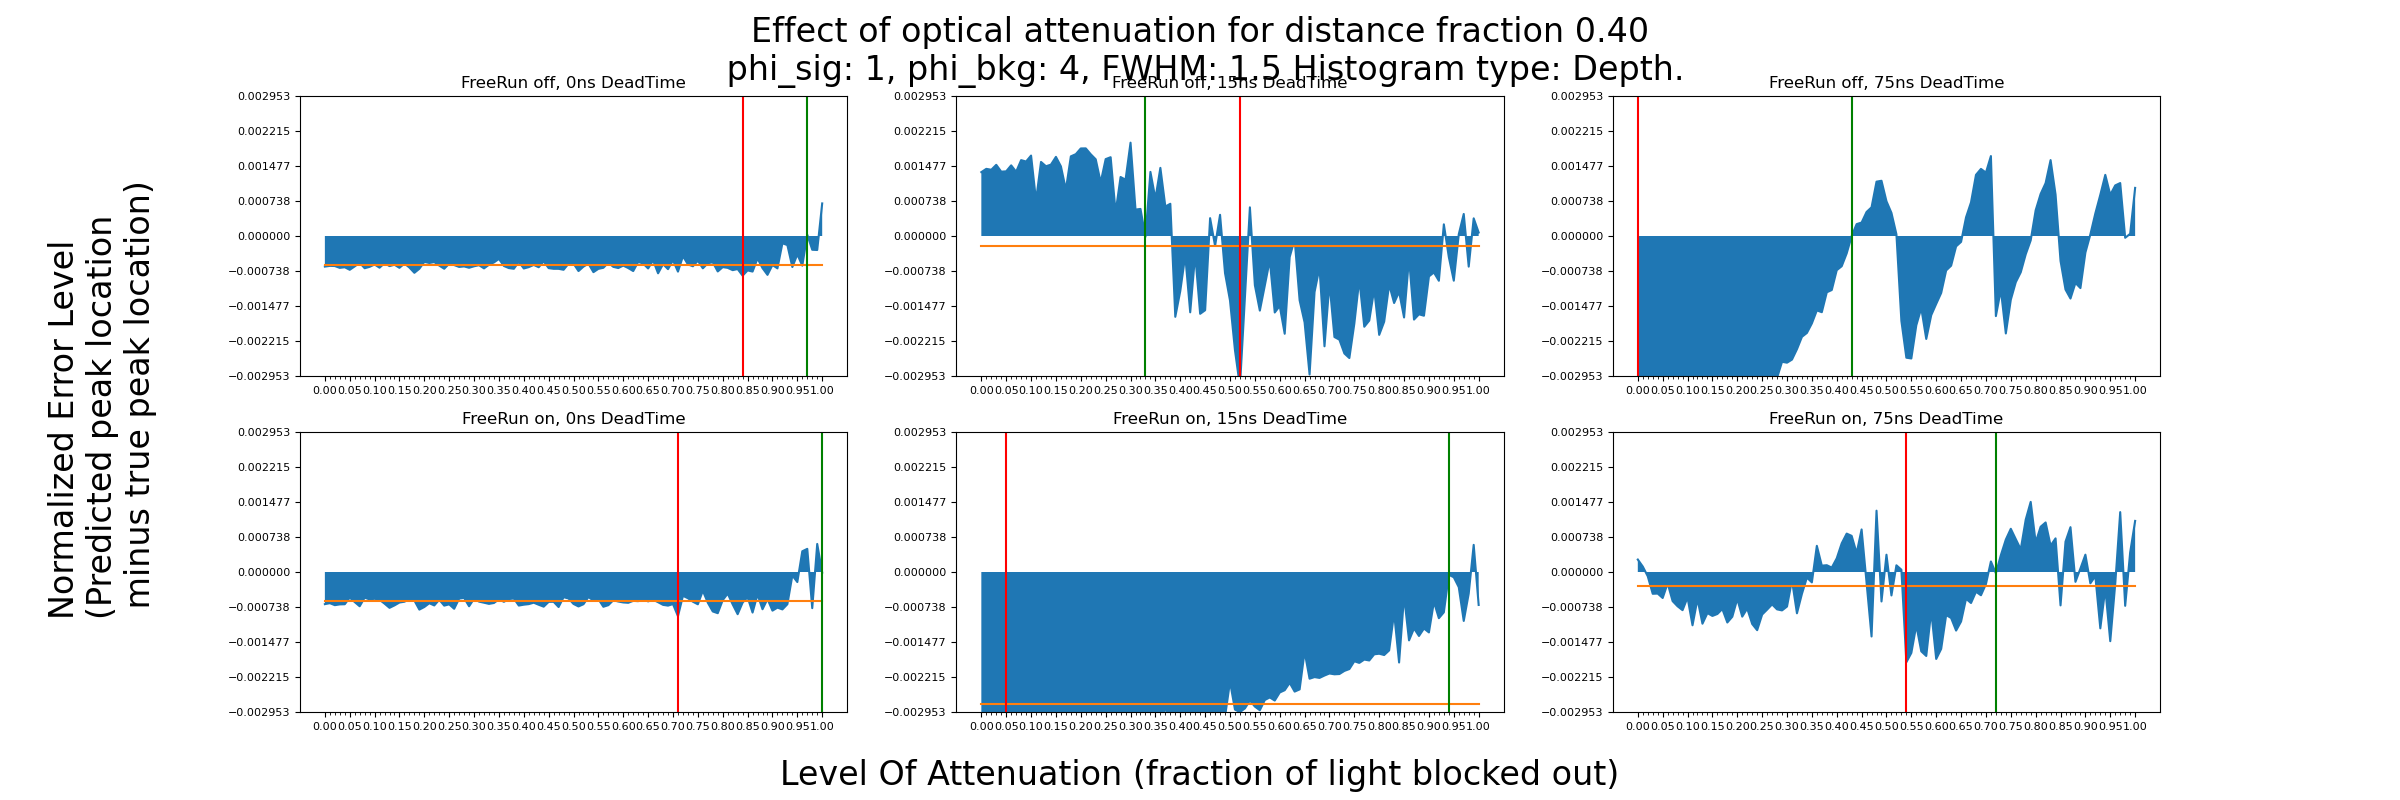
\includegraphics[width=1\linewidth]{sharedFreeExample.png}
      \label{fig:sharedExample}
    \end{subfigure}
    \caption{\label{fig:freerunComparsion}Freerun and non-Freerun on different y axes.}
  \end{figure}
\end{frame}

\begin{frame}
  \begin{figure}[H]
    \centering
    \begin{subfigure}[b]{1\textwidth}
      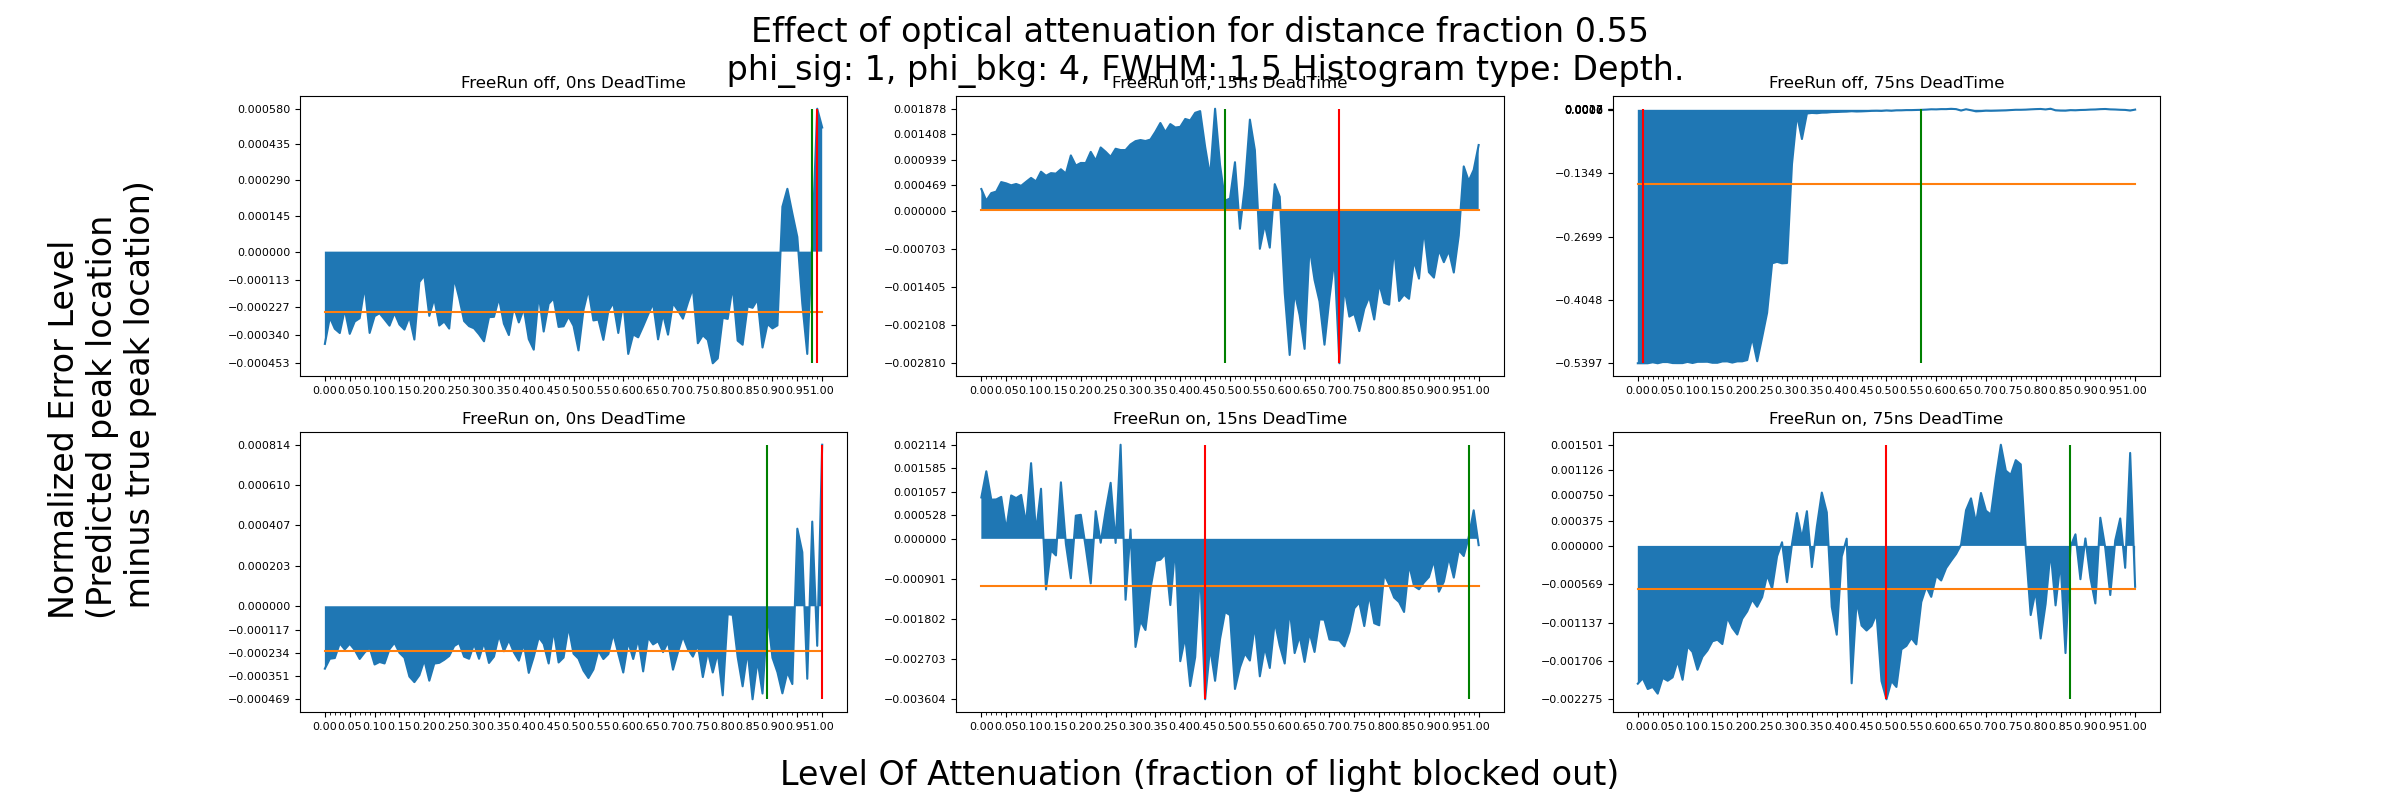
\includegraphics[width=1\linewidth]{1.5Example.png}
      \label{fig:1.5Example}
    \end{subfigure}
    \begin{subfigure}[b]{1\textwidth}
      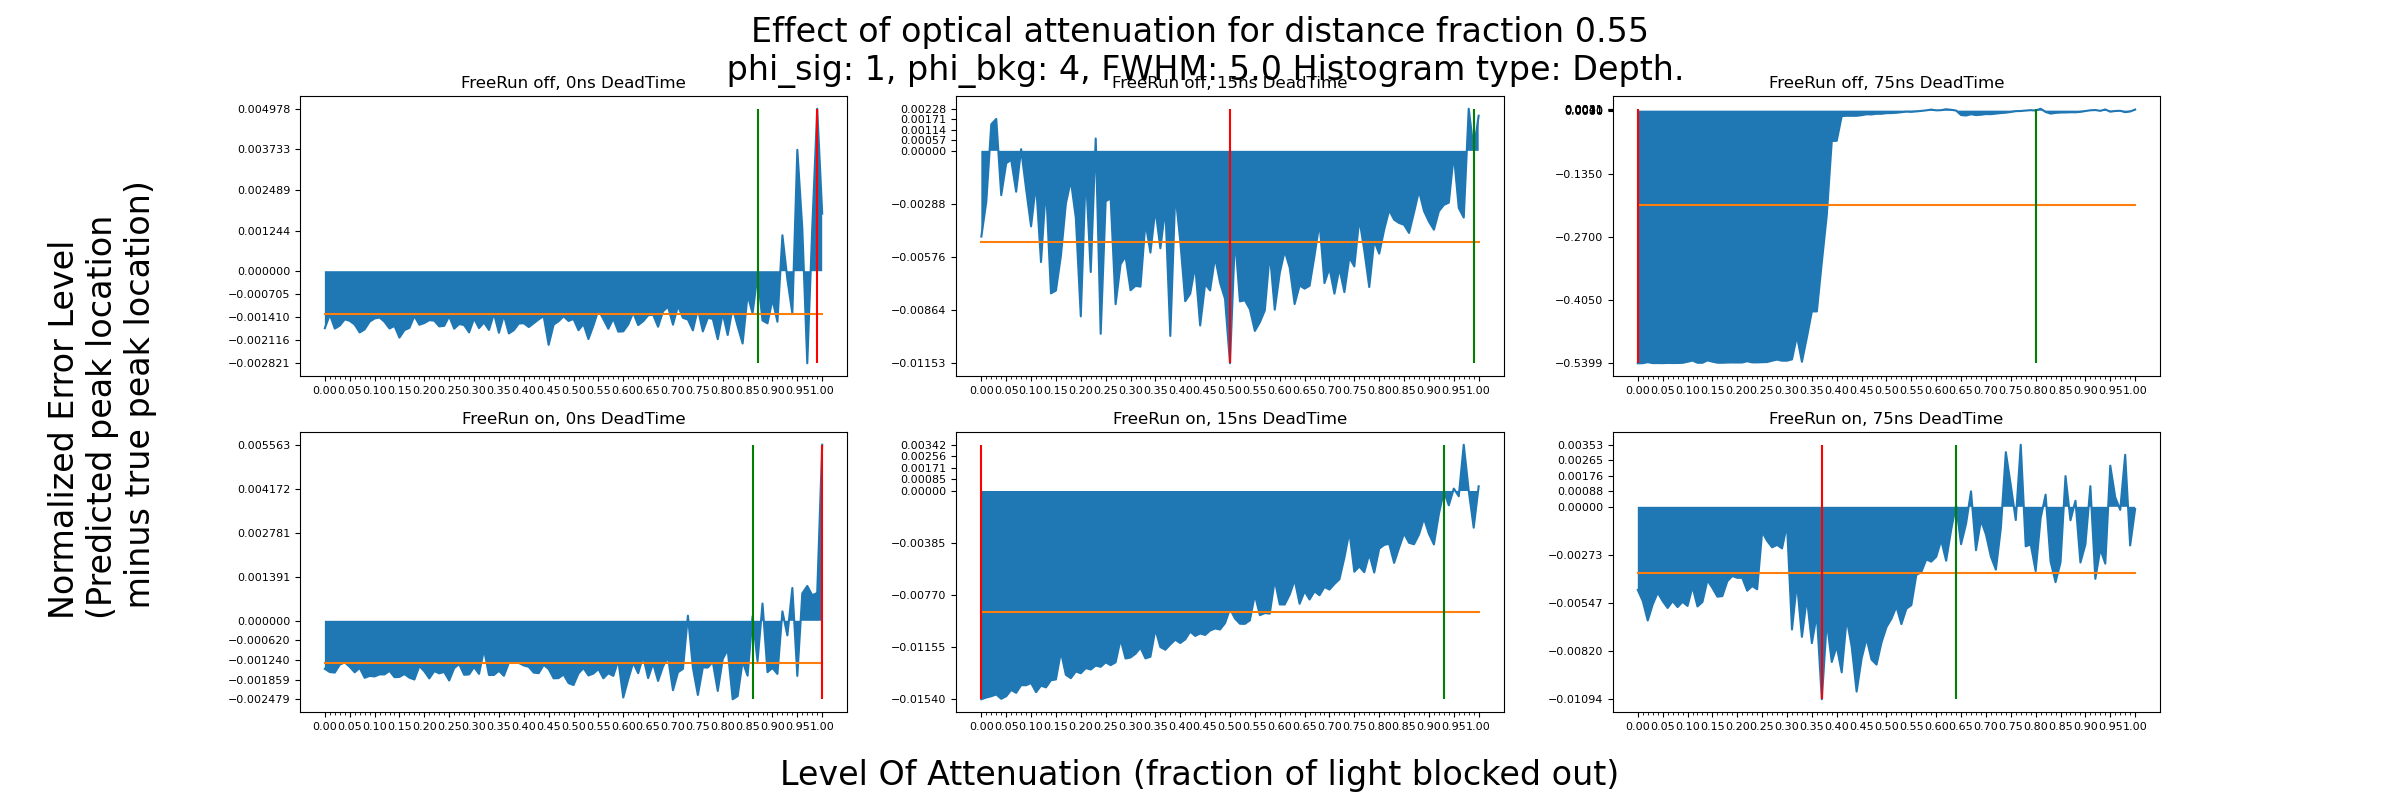
\includegraphics[width=1\linewidth]{5.0Example.png}
      \label{fig:5.0Example}
    \end{subfigure}
    \caption{\label{fig:pulseComparison}1.5 FWHM vs 5.0 FWHM.}
  \end{figure}
\end{frame}

\begin{frame}
  \center{\bfseries{Discussion and Analysis of data}}
\end{frame}

\begin{frame}
  In Short, the results show that:
  \begin{itemize}
  \item EDH Error Calculation produces more error than EWH Error Calculation, which does not support my hypothesis that EDH Error Calculation produces less error than EWH Error Calculation.
  \item FreeRun simulations produce less error than Non-Freerun simulations, which does support my hypothesis that FreeRun (asynchronous) simulations produce less error than Non-Freerun (parallel) simulations.
  \item 1.5 FWHM simulations produce less error than 5.0 FWHM simulations, which does not support my hypothesis that FreeRun simulations produce less error than Non-Freerun simulations.
  \end{itemize}
\end{frame}

\begin{frame}
  While some of these results were different from my expectations, they are still explainable observations. Some \underline{possible (but not necesarily correct)} explanations are as follows:
  \begin{itemize}
  \item EDH error calculation may be prone to overvaluing shorter but wider peaks like the ones produced by skewed data and undervaluing tall but thin peaks like the ones produced at the actual peak, while EWH error calculation simply measures the highest bucket.
  \item FreeRun simulations are less prone to producing skewed data, as the point where individual detectors start detecting photons within a cycle varies, thus allowing photons from later into each cycle hit the detector more often.
  \item shorter FWHM simulations may produce taller, thinner peaks as the photons are clustered closer together, thus making the peak stand out from the rest of the data better.
  \end{itemize}
\end{frame}

\begin{frame}
  My findings have a few implications for practial use of SPCs. The specific implications is that when trying to minimize error while taking SPC photographs...
  \begin{itemize}
  \item One should use EWH error caclulation instead of EDH error calculation.
  \item One should use Asynchronous data collection (Freerunningmode) instead of Parallel data collection.
  \item One should set their laser's FWHM to 1.5 instead of 5.0.
  \end{itemize}
\end{frame}

\begin{frame}
  \center{\bfseries{FLAWS AND LIMTIS}}
\end{frame}

\begin{frame}
  All data was collected using the SPCSimLib library, so any flaws in the methods by which it collects data would cause flaws in the data I analyzed and graphed. Additionally, each simulation was prone to it's own fluctuations, and while I did take an average of 10 repetitions to reduce the error in my error measurements (meaning the difference between my average error measurements and base reality) there were still fluctuations in the data, despite the relatively clear trends.
\end{frame}

\begin{frame}
  \center{\bfseries{CONCLUSIONS}}
\end{frame}

\begin{frame}
   As Single Pixel Cameras develop and their use increases, it is important to know what settings will allow said SPCs to produce the most accurate pictures.
  \begin{itemize}
  \item I found that calculating error with EWH error calculation, using Asynchronous Data Collection and 1.5 FWHM lasers produced the most accurate results.
  \item This implies that to produce highly-accurate pictures for SPC cameras, one should use said settings.
  \item From this, I propose that these become standard settings for SPC cameras.
  \item I also suggest that more research be done into FWHM to figure out the optimal FWHM.
  \end{itemize}
\end{frame}

\begin{frame}
  \center{\bfseries{BIBLIOGRAPHY}}
\end{frame}

\begin{frame}
  \printbibliography
  
\end{frame}

\end{document}
